\documentclass[angelino.tex]{subfiles} 

\begin{document}
In Bayesian inference with MCMC, the target density is a
(possibly unnormalized) posterior distribution.
In most modeling problems, %such as those corresponding to graphical models,
the target density can be decomposed into a product of terms.
If the data~$\x = \{x_n\}_{n=1}^N$ are conditionally independent given the model
parameters~$\theta$, there is a factor for each of the~$N$ data:
\begin{align}
\pi(\theta \given \x) &\propto \pi_0(\theta) \,\pi(\x \given \theta) 
                 = \pi_0(\theta) \prod_{n=1}^{N} \pi(x_n \given \theta).
\label{eq:poserior}
\end{align}
Here~$\pi_0(\theta)$ is a prior distribution and~$\pi(x_n\given\theta)$
is the likelihood term associated with the~$n$th datum.
The logarithm of the target distribution is a sum of terms,
\be
\mcL(\theta) = \log \pi(\theta \given \x)
= \log \pi_0(\theta) + \log \pi(\x \given \theta) + c
= \log \pi_0(\theta) + \sum_{n=1}^{N} \log \pi(x_n \given \theta) + c\,,
\label{eq:log-posterior}
\ee
where~$c$ is an unknown constant that does not depend on~$\theta$
and can be ignored.
Our predictive prefetching algorithm uses this to form
predictors~$\Predictor{\rho}$ as in Equation~\ref{eqn:estimator}.
We can reframe~$\Predictor{\rho}$ using log probabilities as
\be
    \Predictor{\rho} \approx \Pr\left(\log \gamma_\rho < \mcL(\theta') - \mcL(\theta)\right),
\ee
where~$\gamma_\rho$ is the precomputed random MH threshold of
Equation~\ref{eqn:precomputed-threshold}.  
One approach to forming this predictor is to use a normal model
for each~$\mcL(\theta)$, as done by~\citet{korattikara-2014-austerity}.
However, rather than modeling~$\mcL(\theta)$ and~$\mcL(\theta')$ separately,
we can achieve a better estimator with lower variance by considering them
together.  Expanding each log likelihood gives:
\begin{align}
\mcL(\theta') - \mcL(\theta) &= \log\pi_0(\theta') - \log\pi_0(\theta) + \sum_{n=1}^N\Delta_n\\
\Delta_n &= \log\pi(x_n\given\theta') - \log\pi(x_n\given\theta)\,.
\label{eqn:difference}
\end{align}
In Bayesian posterior sampling, the proposal $\theta'$ is usually a perturbation
of~$\theta$ and so we expect~$\log \pi(x_n\given \theta')$ to be correlated
with~$\log \pi(x_n \given \theta)$.
%Figure~\ref{correlation} illustrates this through an empirical example
%with a scatterplot of~$\log \pi(x_i | \theta')$ versus~$\log \pi(x_i | \theta)$.
In this case, the differences~$\Delta_n$ occur on a smaller scale than they
would otherwise and also have a smaller variance compared to the variance
of~$\log \pi(x_n \given \theta)$ across data terms.
%We depict this in Figure~\ref{histogram}, using the same example,
%this time plotting histograms of~$\log \pi(x_i | \theta)$ at
%the current state~(top) and~$\log \pi(x_i | \theta)$ at the proposal~(middle),
%as well as the differences~$\Delta_i$~(bottom).
%Consistent with the previous scatterplot, the histograms
%of~$\log \pi(x_i | \theta')$ and~$\log \pi(x_i | \theta)$
%are very similar, but their empirical standard deviations are
%more than 30 times greater than that of the differences~$\Delta_i$.
%
%\begin{figure}[t!]
%\begin{center}
%\includegraphics[width=0.8\textwidth]{figs/correlation.png}
%\end{center}
%\caption{Scatterplot of~$\log \pi(x_i | \theta')$ versus~$\log \pi(x_i | \theta')$.
%In Bayesian posterior sampling,
%the likelihood decomposes into per-datum contributions.
%Evaluated at the current state~$\theta$ and proposal~$\theta'$,
%these are~$\log \pi(x_i | \theta)$ and~$\log \pi(x_i | \theta')$, respectively.
%For each datum~$x_i$, these terms are highly correlated.
%Depicted is an example % from our multinomial logistic regression model
%with~${N = 50,000}$ data items, where the correlation coefficient is measured
%to be greater than~$0.999$.
%The dashed line corresponds to the identity.}
%\label{correlation}
%\end{figure}
%
%\begin{figure}[t!]
%\begin{center}
%\includegraphics[width=0.8\textwidth]{figs/histogram.png}
%\end{center}
%\caption{Histograms of per-datum contributions to the likelihood,
%$\log \pi(x_i | \theta)$ at the current state~(top, $s=45.69$)
%and~$\log \pi(x_i | \theta)$ at the proposal~(middle, $s=45.95$),
%as well as the differences
%$\Delta_i = \log \pi(x_i | \theta') - \log \pi(x_i | \theta)$
%corresponding to the Metropolis-Hastings ratio (bottom, $s=1.48$).
%We use $s$ to denote the empirical standard deviation.
%Each histogram has 100 bins; the large bars near zero are explained by
%data items that happened to be classified correctly with high confidence by
%the multinomial logistic regression model.}
%\label{histogram}
%\end{figure}

A concrete sequence of estimators is obtained by subsampling the differences.
%
Let $\{\Delta_n\}_{n=1}^{m}$ be a subsample of size~${m<N}$, without
replacement, from $\{\Delta_n\}_{n=1}^{N}$.  This subsample can be used to
construct an unbiased estimate of~${\mcL(\theta') - \mcL(\theta)}$.
%
We model the terms of this subsample as i.i.d. from a normal distribution with
bounded variance $\sigma^2$, leading to:
%
\begin{align}
  {\mcL(\theta') - \mcL(\theta)} &\sim \N(\hat{\mu}_m, \hat{\sigma}_m^2)\,.
\label{model-single}
\end{align}
%
The mean estimate $\hat\mu_m$ is empirically computable:
%
\begin{align}
  \hat{\mu}_m &= \log \pi_0(\theta') - \log\pi_0(\theta) + \frac{N}{m}\sum_{n=1}^m \Delta_n\,.
  \label{eqn:mu}
\end{align}
%
The error estimate $\hat\sigma_m$ may be derived from $s_m/\sqrt{m}$, where $s_m$ is the empirical standard deviation of the~$m$ subsampled~$\Delta_n$ terms. To obtain a confidence interval for the sum of~$N$ terms, we multiply this estimate by~$N$ and the finite population correction~$\sqrt{(N - m) / N}$, giving:
\begin{align}
\hat{\sigma}_m = s_m  \sqrt{\frac{N (N - m)}{m}}\,.
\label{eqn:sigma}
\end{align}
%
\begin{figure}[t!]
\vspace{-0.2in}
\begin{center}
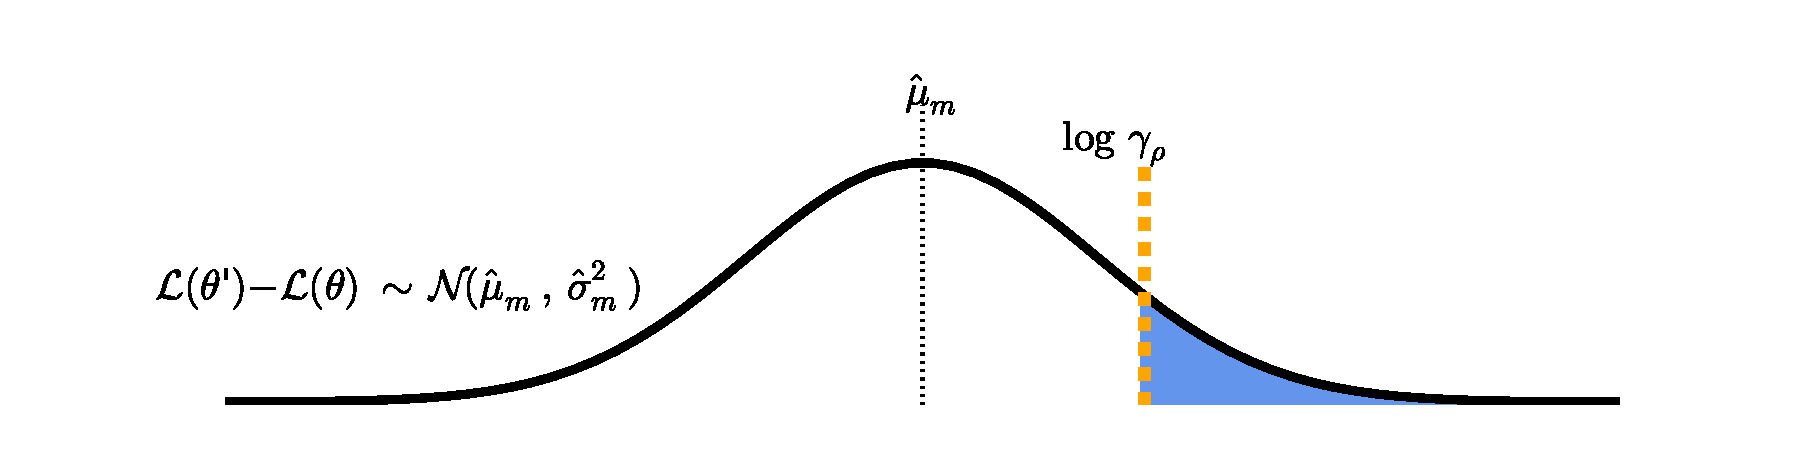
\includegraphics[width=\textwidth]{figs/accept.pdf}
\end{center}
\vspace{-0.2in}
\caption{We use a normal model for the difference of log posteriors at states~$\theta'$ 
and~$\theta$ as~${\mcL(\theta') - \mcL(\theta)} \sim \N(\hat{\mu}_m, \hat{\sigma}_m^2)$.
Thus, the predictor~$\PredEst{\rho}{m}$ is equal to the area under~$\N(\mu, \sigma^2)$
to the right of~$\log \gamma_\rho$.
Recall that~$\gamma_\rho$ is the precomputed random MH threshold of
Equation~\ref{eqn:precomputed-threshold} and depends on a
uniform random variate~${u \sim \Unif(0, 1)}$.
}
\label{fig:accept}
\end{figure}
%
\noi As illustrated in Figure~\ref{fig:accept}, we can now form the
predictor~$\PredEst{\rho}{m}$ by considering the tail probability
for~$\log \gamma_\rho$, where recall~$\gamma_\rho$ is defined in
Equation~\ref{eqn:precomputed-threshold}:
\begin{align}
\PredEst{\rho}{m} &= \int^\infty_{\log \gamma_\rho}
\N(z\given \hat{\mu}_m, \hat{\sigma}_m^2)\,\mathrm{d}z\\
&= 1 - \int_{-\infty}^{\log \gamma_\rho} \N(z\given \hat{\mu}_m, \hat{\sigma}_m^2)\,\mathrm{d}z \nn \\
&=\frac{1}{2} \left[
1 - \erf\left( \frac{\log \gamma_\rho - \log\hat{\mu}_m}{\sqrt{2}\hat{\sigma}_m}\right)
\right] \nn \\
&= \frac{1}{2}\left[
1 + \erf\left( \frac{\log\hat{\mu}_m - \log \gamma_\rho}{\sqrt{2}\hat{\sigma}_m}\right)
\right]\,.
\label{eqn:subset}
\end{align}

\end{document}
